\section{Adiabatic Quantum Computation}
\label{Section:AQC}
{\color{blue}ALAN: Talk here about adiabatic theorem and evolutions. Then, introduce the concept/definition of
adiabatic quantum computation, where we define the problem Hamiltonians and etc. To this end,
we can get results by Sarandy [https://doi.org/10.1007/s11128-004-7712-7] and references therein,
and some discussion done in [Rev. Mod. Phys. 90, 015002 (2018)] to make our life easier.}

The adiabatic theorem of quantum mechanics provides the foundation for an alternative model
of quantum computation based on continuous-time evolution. Consider a time-dependent Hamiltonian
$H(t)$ with a discrete and non-degenerate spectrum. Thus we can define its instantaneous
eigenstates and eigenenergies by
\begin{equation}
    H(t) \ket{n(t)} = E_n (t) \ket{n(t)}.
    \label{eq:instantaneous_eigenstates}
\end{equation}

\noindent The adiabatic theorem states that a quantum system initially prepared in an eigenstate
$\ket{n(0)}$ of  $H(0)$, will remain in its instantaneous eigenstate $\ket{n(t)}$ throughout
the evolution, provided that the spectrum remains gapped and the change is sufficiently
slow~\cite{sarandy_consistency_2004,albash_adiabatic_2018}. This last condition is generally formulated as follows:
\begin{equation}
    \max_{0 \leq t \leq T} \bigg| \dfrac{\bra{k} \dot{H} \ket{n}}{g_{nk}} \bigg| \ll \min_{0 \leq t \leq T} \big| g_{nk} \big|,
    \label{eq:adiabatic_condition}
\end{equation}
where $T$ is the total evolution time and $g_{nk}$ represents the energy gap between levels $n$ and $k$: 
\begin{equation}
    g_{nk}(t) \equiv E_n(t) - E_k(t)
    \label{eq:energy_gap}
\end{equation}

Despite the adiabatic theorem works for any eigenstate, in practice it is customary to focus on
ground state adiabatic passages. This is because ground states are typically more robust against
decoherence and thermal excitations, as they are energetically isolated from higher-energy levels.
Moreover, for many computational problems, particularly those related to optimization problems,
it is possible to construct a problem Hamiltonian $H_\mathrm{P}$ whose ground state encodes
the solution to the instance under consideration.

\begin{figure}[h]
    \centering
    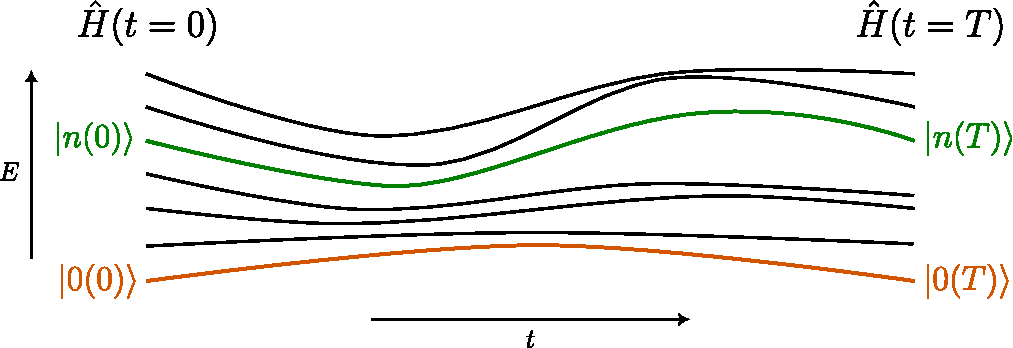
\includegraphics[width=0.75\textwidth]{01-introduction/figs/adiabatic_theorem.pdf}
    \caption{Schematic of an adiabatic passage. The orange line represents the Hamiltonian's ground state, while
    the green a Hamiltonian's eigenstate different from the ground state.}
    \label{fig:adiabatic_passage}
\end{figure}

In the adiabatic quantum computation model, the Hamiltonian is interpolated between an
initial Hamiltonian $H_0$, with a known and easily preparable ground state, and the problem
Hamiltonian $H_\mathrm{P}$, according to a schedule~\cite{albash_adiabatic_2018}:
\begin{equation}
    H(t) = \big[1 - s(t)\big] H_0 + s(t) H_\mathrm{P}, \quad s(t) \in [0,1],
    \label{eq:adiabatic_passage}
\end{equation}
where $s(t)$ is a smooth, monotonic function such that $s(0)=0$ and $s(T)=1$. The problem
Hamiltonian $H_\mathrm{P}$ is designed so that its ground state corresponds to the solution
of the computational task.

{\color{red}(Maybe talk about AQC can be efficiently simulated in the circuit model).}

\subsection{Adiabatic Quantum Annealers}

{\color{blue}ALAN: Here we discuss about the adiabatic quantum annealers, where the problem Hamiltonian
is the Ising Hamiltonian (which is the focus of our applications). To this end, maybe we can use the
review paper to get some key discussions [Rev. Mod. Phys. 90, 015002 (2018)].}

An important and widely studied application of adiabatic evolution in quantum
devices is Adiabatic Quantum Annealing (AQA), where the goal is to find low-energy configurations of
a classical cost function mapped onto a quantum Hamiltonian. AQA is most often applied to Quadratic Unconstrained
Binary Optimization (QUBO) problems, which can be exactly reformulated as a 2-body interaction Ising
Hamiltonian of the form
\begin{equation}
    H_\mathrm{P} = \sum_i h_i \sigma_i^z + \sum_{i<j} J_{ij} \sigma_i^z \sigma_j^z\,,
    \label{eq:ising_hamiltonian}
\end{equation}
where $h_i$ are local fields, $J_{ij}$ represent coupling strengths between qubits, and
$\sigma_i^z$ are Pauli-Z operators acting on the $i$-th qubit. The task is to drive the system
from an initial, easily preparable ground state towards the ground state of $H_\mathrm{P}$,
which encodes the optimal solution to the problem at hand.

In a typical AQA protocol, the evolution begins with an initial transverse-field Hamiltonian
\begin{equation}
    H_0 = \sum_i \sigma_i^x\,.
    \label{eq:transverse_field_hamiltonian}
\end{equation}
whose ground state is straightforward to prepare. The system is then evolved according to the interpolation
scheme in equation (\ref{eq:adiabatic_passage}). The aim is to adiabatically steer the system from the easily
preparable ground state $H_0$ to the ground state of $H_\mathrm{P}$, which encodes the solution to the
problem of interest.

This procedure is straightforward for problems that can be expressed in the QUBO form, as they can be mapped to
an Ising Hamiltonian with only two-body interactions. However, the factorization problem presented in
chapter~\ref{Chapter:Factorization} does not directly fall into the QUBO class, as its Hamiltonian contains
three- and four-body interaction terms. As will be discussed later, this limitation can be addressed by adopting
an alternative formulation of the problem Hamiltonian that avoids these high-order terms while preserving the encoded solution.